\documentclass{standalone}
\usepackage{tikz}
\usepackage{amsmath}

\begin{document}

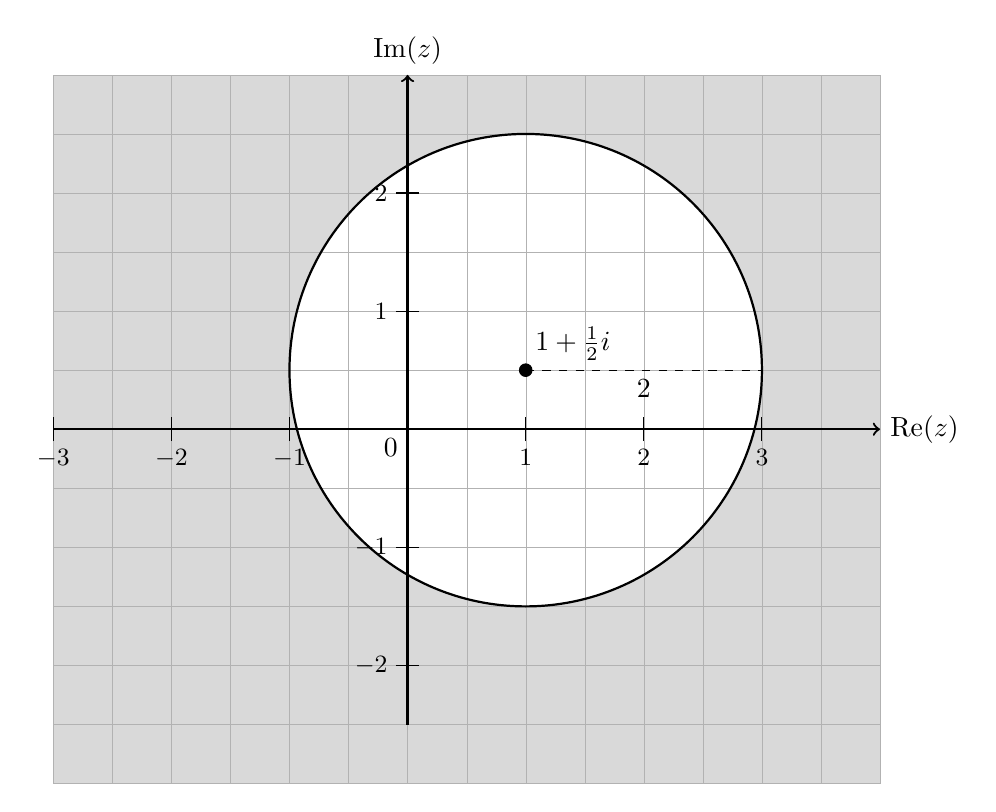
\begin{tikzpicture}[scale=1.5]
    
    % Center of the circle
    \coordinate (center) at (1, 0.5);

    % Fill outside region
    \begin{scope}
        \clip (-3, -3) rectangle (4, 3);
        \fill[gray!30] (-3, -3) rectangle (4, 3);
        \fill[white] (center) circle (2);
    \end{scope}

    % Draw grid
    \draw[step=0.5, gray!60, ultra thin] (-3, -3) grid (4, 3); % Visible grid with lighter color
    
    % Circle
    \draw[thick] (center) circle (2);
    
    % Center point
    \filldraw[black] (center) circle (1.5pt) node[above right] {$1 + \frac{1}{2}i$};
    
    % Radius line
    \draw[dashed] (center) -- ++(2, 0) node[midway, below] {$2$};
    
    % Axes
    \draw[->, thick] (-3, 0) -- (4, 0) node[right] {$\text{Re}(z)$};
    \draw[->, thick] (0, -2.5) -- (0, 3) node[above] {$\text{Im}(z)$};

    % Axis ticks
    \foreach \x in {-3, -2, -1, 1, 2, 3}
        \draw (\x, -0.1) -- (\x, 0.1) node[below=8pt] {\small $\x$};
    \foreach \y in {-2, -1, 1, 2}
        \draw (-0.1, \y) -- (0.1, \y) node[left=8pt] {\small $\y$};

    % Labels for axes
    \node[below left] at (0, 0) {$0$};

\end{tikzpicture}

\end{document}

